\documentclass[../Relazione.tex]{subfiles}

\begin{document}

\section{Simulazione del sistema con CPN Tools}
Di seguito vengono riportati i risultati della simulazione  dell'\textbf{intero sistema} effettuata tramite \textit{CPN Tools}. I parametri della simulazione sono quelli standard indicati dalla consegna: \textbf{30 subruns} dove, ognuna di queste,  corrisponde ad uno scenario di \textbf{5 giorni} in cui vengono commesse \textbf{40 violazioni al giorno}.

    \begin{figure}[!h]
        \captionsetup{singlelinecheck = false, format= hang, justification=raggedright, font=footnotesize, labelsep=space}
        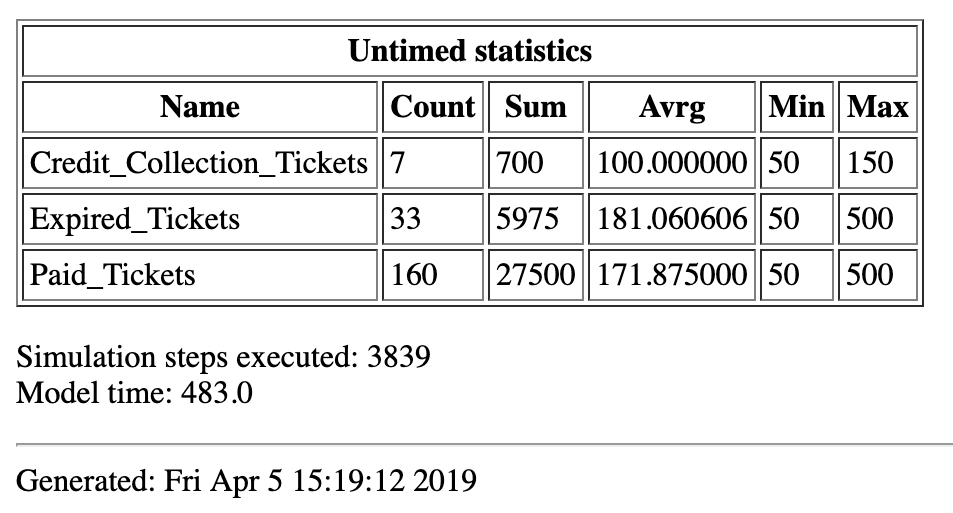
\includegraphics[scale=0.55]{ATCS/simulations/PerfSummary.png}
        \caption{Sommario della simulazione}
        \label{fig:PerfSummary}
    \end{figure}
    
    \begin{figure}[!h]
        \centering
        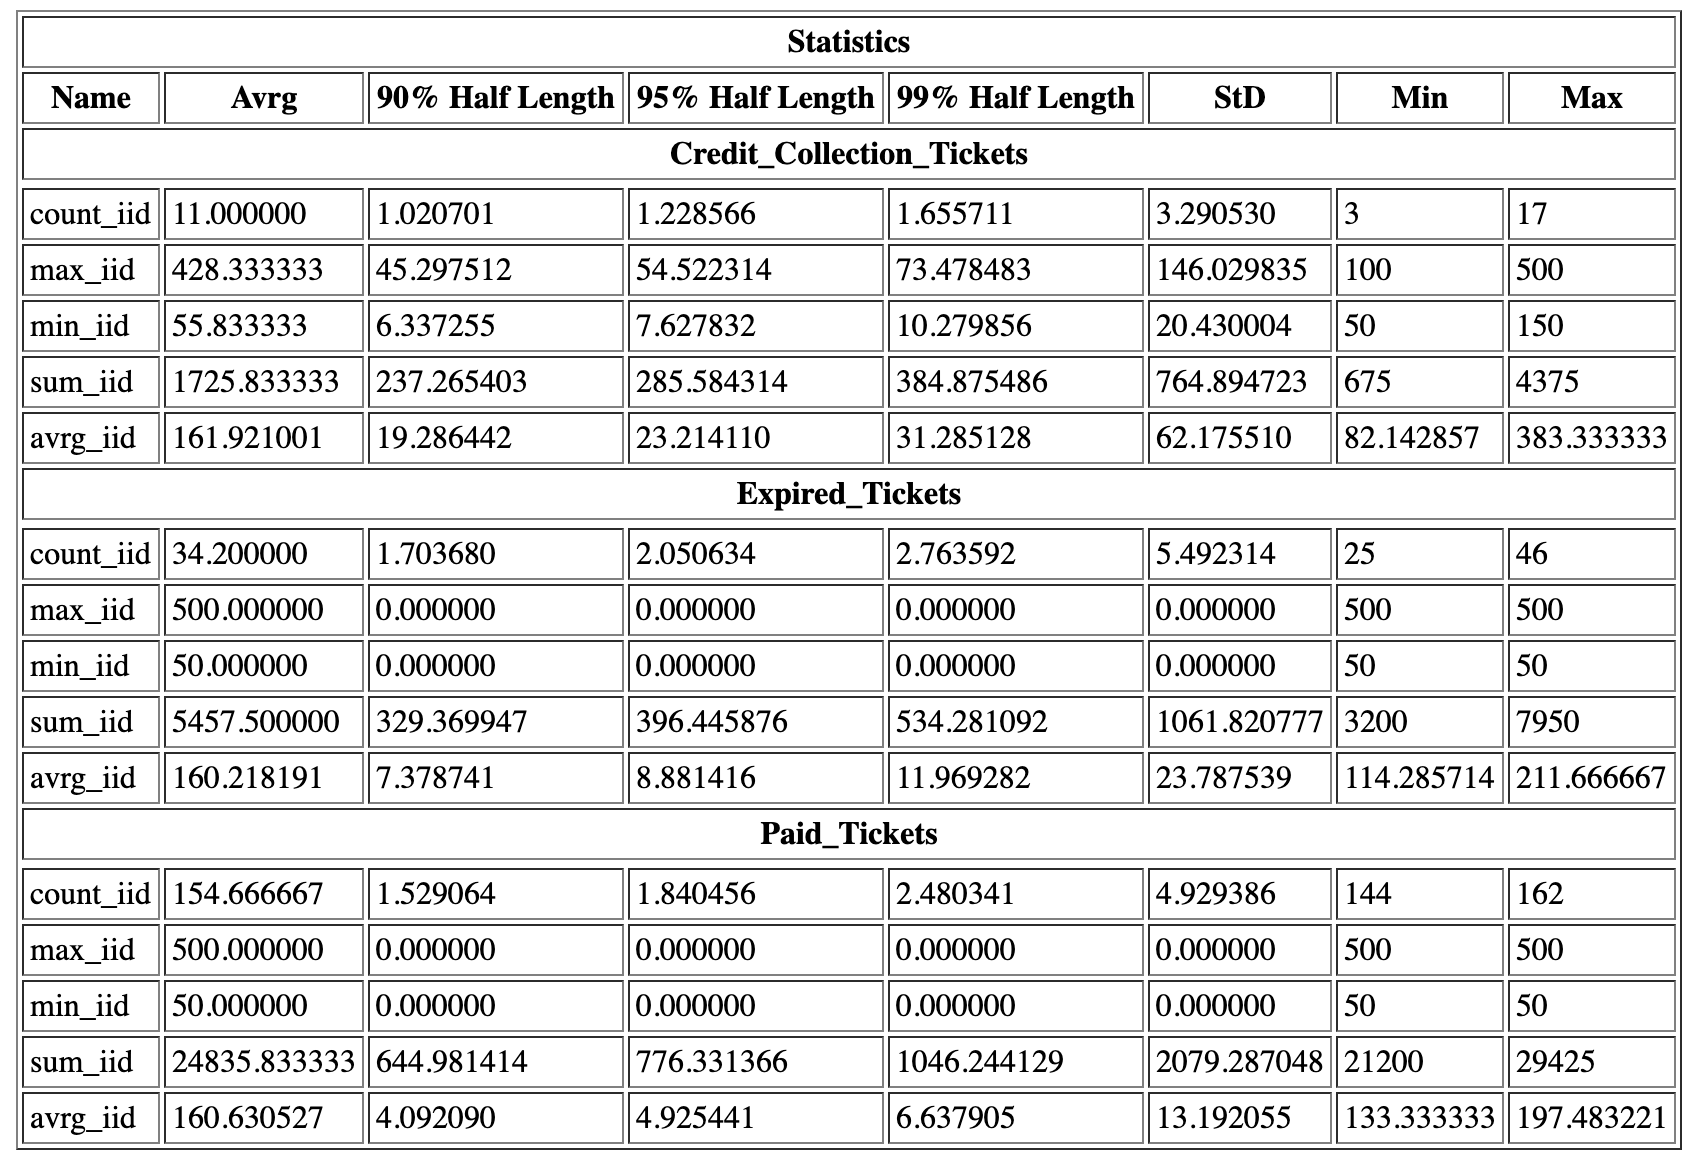
\includegraphics[scale=0.55]{ATCS/simulations/PerfReport.png}
        \caption{Performance Simulation - Report completo}
        \label{fig:PerfReport}
    \end{figure}
    
\end{document}
		